\chapter{Introduction}
\label{chap:introduction}
\minitoc

\ac{AD} and anomaly localization in medical images refer to the process of identifying abnormal areas or regions within images of various modalities, one of which is Magnetic Resonance Imaging (MRI) scans. Fully supervised deep learning approaches have demonstrated robust performance in assisting radiologists with MRI interpretation and automating tasks such as anomaly segmentation. For example, UNet-based algorithms have significantly contributed to advancements in automatic lesion segmentation. However, these methods require large datasets with image-level labels and pixel-level annotations for training, which are typically expensive and time consuming to obtain. Furthermore, the subtle nature of certain anomalies makes them difficult to detect, even for human experts. Consequently, rare and subtle anomalies may be underrepresented or entirely absent from training datasets, reducing the robustness of supervised approaches. An alternative is \ac{UAD}, which relies solely on healthy data rather than annotated pathological examples. The objective is to learn the underlying distribution of healthy brain MRI scans, and then to detect anomalies as deviations from this learned distribution. In recent study, \cite{lagogiannisUADStudyOfSOTA} categorize UAD methods into four groups: image reconstruction-based, feature-modeling, attention-based and self-supervised anomaly detection methods. In this project, we will focus on the reconstruction-based method, in particular using diffusion models. Additionally, longitudinal data in MRI scans provide repeated measurements of the same subject over time, offering valuable insights into disease progression and temporal patterns. In the context of \ac{UAD}, most \ac{DMs} treat each image independently (spatial dimension), without considering longitudinal dependencies (temporal dimension). Our goal is to investigate the viability of leveraging additional information provided by longitudinal data. Our source code is available at \url{https://github.com/khuongdb/spatio-temporal-DM}\footnote{At the time of writing, we are still developing and expanding the project. The source code is not yet fully refined.}.  

\section{Reconstruction-based UAE with diffusion models}
\label{sec:introduction-sdm}

\begin{figure}
    \centering
    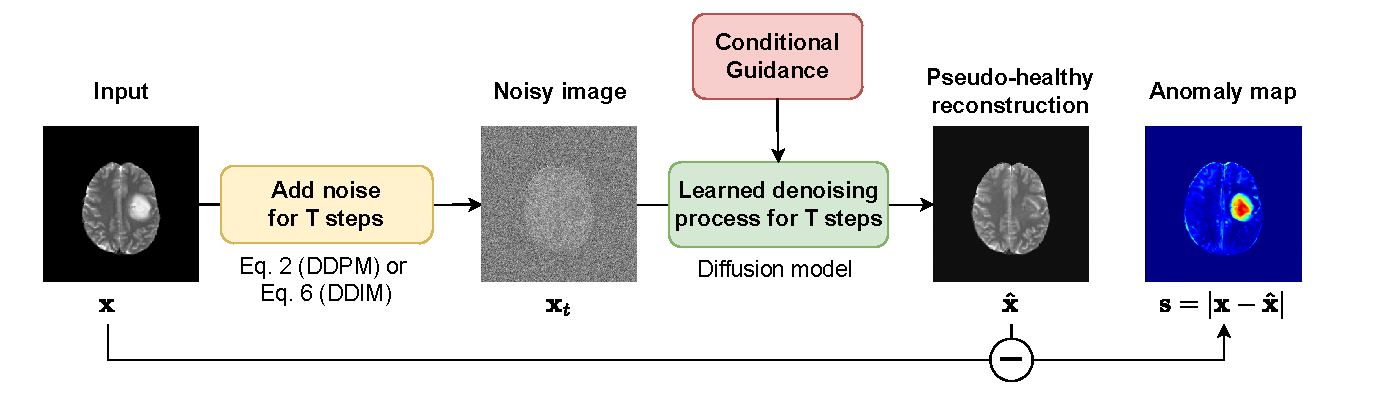
\includegraphics[width=1\linewidth]{figures/uad-overview.pdf}
    \caption[Overview of reconstruction-based UAD]{Overview of reconstruction-based anomaly segmentation with diffusion models. During training, the model learns the distribution of healthy dataset. At inference, we translate an input image to its pseudo-healthy counterpart $\hat\rvx$. The pixel-wise anomaly score map is given by the difference between input and output $D_p = |\rvx - \hat\rvx|$. Figure from \cite{berceaDDPMforMedicalImagesStudy2024}}
    \label{fig:general-uad-diffusion-methods}
\end{figure}

In reconstruction-based \ac{UAD}, a model is trained exclusively on healthy data and, during inference, attempts to generate a pseudo-healthy version of the input image. The core assumption is that since the model has only seen healthy examples during training, it will fail to accurately reconstruct pathological regions while still producing realistic healthy structures. The discrepancy between the input and its pseudo-healthy reconstruction is used to generate a residual map, where high error values indicate potential anomalies. The residual error map is often quantified using the pixel-wise $l$1-error: $D_p = | \rvx - \hat\rvx |$. \ac{GMs} known for their impressive ability to synthesize realistic images, have become prominent tools in this domain. In particular, \ac{VAE} \cite{zimmerer2019VAE-UAD} and \ac{GAN} \cite{fAnoGAN} have been explored, as well as their variants. Recently, \ac{DMs} have shown promise as generative models for \ac{UAD}, due to their ability to produce high resolution synthesized images with accurate inpainting \cite{pinaya2022fastUAD-DDPM, wolleb2022DDPM-weaksupervise, behrendt2025cDDPM}. \cref{fig:general-uad-diffusion-methods} shows an overview of anomaly segmentation task with diffusion models. Nevertheless, reconstruction-based \ac{UAD} methods in general and diffusion models in particular face some critical challenges, mainly:

\begin{description}
    \item[Reconstruction quality]: even though generative models can produce very high quality samples, it is very unlikely that we can achieve near-exact reconstruction images, even those of healthy subjects. This introduces many false positive regions in our anomaly map, specially small errors in the background and around sharp edges of the object. This underlines the importance of developing models that can distinguish between residual errors caused by anomalies and those caused by model limitations.
    
    % As a consequence, selecting an appropriate threshold remains a critical and ongoing challenge for binarizing the anomaly score map to have accurate segmentation without false positive. 
    
    \item[Structure preservation]: in diffusion model, we gradually add noise to input image (\emph{forward process}) and remove them to recover healthy image (\emph{denoise process}). The quantity and quality of noise added to image plays a crucial role in diffusion process, and this aspect is well studied in the literature. \cite{behrendt2025cDDPM} highlight that a key challenge is to limit the reconstruction to healthy brain anatomy. On the one hand, we want to avoid models with limited reconstruction accuracy, which produce imperfect reconstructions everywhere. On the other hand, models that generate highly accurate reconstructions tend to perform a "copy task", resulting in unhealthy structures still reflected in the pseudo-healthy reconstructions. \cite{autoDDPM} refer to this as the \emph{noise paradox}, which states that adding too much noise can destroy not only the anomalous regions but also the healthy structures of the brain. However, adding too little noise can preserve the structure but fail to corrupt the anomaly region, resulting in pseudo-healthy reconstructions that still contain unhealthy structures. 

    \item[Thresholding anomaly score]: Using a trained model, we can produce residual maps that can be interpreted as anomaly scores at both the pixel level and the image level. For anomaly segmentation task, a threshold is required to binarize the score map. At the image level, the goal is to determine a threshold that separates healthy subjects from anomalous ones based on their anomaly scores. However, selecting an appropriate threshold remains an ongoing challenge in \ac{UAD}. Most existing methods in the literature employ greedy algorithms to search for the optimal theoretical threshold based on evaluation metrics (e.g., AUROC, AUPRC). This approach, however, requires a test dataset with fully labeled images and ground-truth segmentations, which violates the principle of unsupervised learning. Other approaches either rely on fixed, predefined threshold values or use quantiles (e.g., the 95th or 97th percentile) of the training or test dataset. In general, selecting an appropriate threshold is challenging and can vary between datasets and applications.
\end{description}

\section{Longitudinal data modeling}
\label{sec:introduction-tdm}

In the context of \ac{UAD} in MRI images, longitudinal data represents repeated MRI scans of a patient at different time points. Unlike timeseries, the number of observations of a single patient is relatively small, and their frequency can be sparse due to patient dropouts, irregular follow-up intervals, and varying lengths of observation periods. Moreover, the complexity of patient metadata, such as age, sex, and disease stage, also affects the progression of disease in different ways. Therefore, we need a solution that can effectively capture both cohort-level (population-wide) and subject-level (individual) trajectories. In recent study, \cite{yangSurveyDiffusionModelsSpatioTemporal2024} show that spatio-temporal diffusion models have achieved state-of-the-art results across many modalities, including images, speech, video, and time series. However, the application of diffusion models to longitudinal data analysis, particularly for MRI anomaly detection, remains underexplored.

Existing literature on longitudinal diffusion models has largely focused on data imputation. However, these approaches rarely exploit the temporal dimension to strengthen spatial anomaly detection. We aim to analyze image sequences across different time points and fuse their information to improve detection and localization of anomalies. This approach can help identify anomalies at earlier stages (reducing false negatives) while filtering out nonpersistent anomalies (reducing false positives). Furthermore, we aim to predict missing observations using the available data and use these imputed images as additional information to improve anomaly localization in future scans.

Our project is inspired by recent advances in longitudinal modeling. \cite{SautyLongitudinalVAE2022} successfully combined a linear mixed-effects model with a \ac{VAE}. In their approach, temporal dependencies are imposed in the latent space of the \ac{VAE}. The mixed-effects model is used to capture the progression of biomarkers in Alzheimer's patients, while spatial variance is learned through the standard \ac{VAE}. By jointly training these two components, their framework demonstrates the ability to model both spatial and temporal aspects in a unified manner. One major difference between these models and diffusion models is that, in \ac{VAE} and normalizing flow frameworks, each observation $\rvx$ corresponds to a single latent variable $\rvz$. Furthermore, this latent variable is typically chosen to have a lower dimensionality, $d \ll D$. In contrast, in diffusion models, each $\rvx$ is associated with a sequence of latent variables $\rvz_t$ that have the same dimensionality as $\rvx$, making it more challenging to impose a temporal structure.

\section{Problem setting}

In this section, we present our problem setting and notations, and we outline the main challenges that we will try to address in this internship. Let ${\rmX^i_{1 \leq i \leq N}}$ be our set of observed $N$ individuals through time, assumed sampled \textit{i.i.d.} from an unknown distribution $p$ that does not depend on $i$. Each patient $i = 1, \ldots , N$ is a sequence of observations through time: $\rvx^i = (\rvx^i_1, \dots, \rvx^i_{L_i})$, where, for each $j, \rvx^i_l \in \mathcal{X} := R^{H \times W \times D}$ is a high dimensional data (2D images or 3D MRI scans) and $L_i$ is the number of observations for a given individual. We note that $L_i \neq L_j$ for any $i \neq j$, which reflects our sparse longitudinal setting: different patients will have different number of observations at different time points. We use notation $L$ to denote longitudinal time point to distinguish from the time step $T$ of diffusion models. 

Given a training set $\mathbf{\mathcal{H} = \{X^{H,i}\}}$ of healthy subjects, our goal is to learn the underlying distribution $q(\rvx^{H, i}_j)$ of each individual sample at any given time. At inference, an anomaly sample $\rvx^{A, i}_j$ is input to our model to produce a pseudo-healthy reconstruction $\hat\rvx^{PH, i}_j$ that follows healthy distribution $q_{\theta}(\rvx^{H, i})$ the network estimates. A residual map is calculated as the difference between original image and its reconstruction $|\rvx - \hat\rvx|$. We will refer to this initial residual map as our pixel-level distance $D_p$ (which can be used for anomaly segmentation). Later on, we will introduce an additional feature distance $D_f$ that focuses more on perceptual difference between two images. 

Our project aims to address some main challenges outlined in \cref{sec:introduction-sdm} and \cref{sec:introduction-tdm}. Our main contributions in this project are summarized as follows: 

\begin{itemize}
    \item Reconstruction quality: we improve the generative power of the diffusion model by enhancing the quality of the conditioning information injected into it. This helps guide the denoising process closer to the true distribution of the input. Secondly, by applying the appropriate noise level, we seek to preserve as much structural detail as possible while ensuring that anomaly regions are fully corrected.
    \item Pixel anomaly score: we introduce feature attention module to combine raw pixel distance with feature distance to further refine our residual map, and eliminate false positive caused by the model errors.
    % We use notation $\rvs$ to denote the anomaly score map, with $\rvs^{pixel}$ and $\rvs^{img}$ represent anomaly score at pixel level and image level, respectively. 
    % \item Image anomaly score: from the pixel anomaly map, we want to find another function to assign a single image anomaly score $\rvs^{img} = \mathcal{F}^{img}(\rvs^{pixel})$. Similarly, this image-level score needs to be thresholded due to the problem of reconstruction quality. 
    \item We employ an automatic thresholding algorithm to remain fully consistent with the unsupervised learning framework.
    \item We incorporate the temporal structure of data to improve the reliability of the spatial diffusion model. Our temporal smoothing module is used to fuse and capture information across different time points. 
    \item When considering the temporal dimension separately, we apply a temporal-aware diffusion model that captures the progression of healthy subjects and generates follow-up images from any given baseline image.
\end{itemize}

% \subsection{Related works}

% \subsubsection{Conditional diffusion models}

% Our project is inspired by recent advances in longitudinal modeling. \cite{SautyLongitudinalVAE2022} successfully combined a linear mixed-effects model with a \ac{VAE}. In their approach, temporal dependencies are imposed in the latent space of the \ac{VAE}. The mixed-effects model is used to capture the progression of biomarkers in Alzheimer's patients, while spatial variance is learned through the standard \ac{VAE}. By jointly training these two components, their framework demonstrates the ability to model both spatial and temporal aspects in a unified manner. One major difference between these models and diffusion models is that, in \ac{VAE} and normalizing flow frameworks, each observation $\rvx$ corresponds to a single latent variable $\rvz$. Furthermore, this latent variable is typically chosen to have a lower dimensionality, $d \ll D$. In contrast, in diffusion models, each $\rvx$ is associated with a sequence of latent variables $\rvz_t$ that have the same dimensionality as $\rvx$, making it more challenging to impose a temporal structure.

% Motivated by the same principle, \cite{ca23LongitudinalNormalizingFlow} use normalizing flow to model the dependencies between observation through time. 

